\subsubsection*{四、设计题}
\setcounter{problemname}{0}

\begin{problem}
分析下图界面,指出其中5处不合理的地方,并指出其违反的2条启发式设计规则,以及该规则的具体内容。请对该界面进行修改,并给出修改后的界面草图。
\begin{figure}[H]
    \vspace{-0.5em}
	\centering
	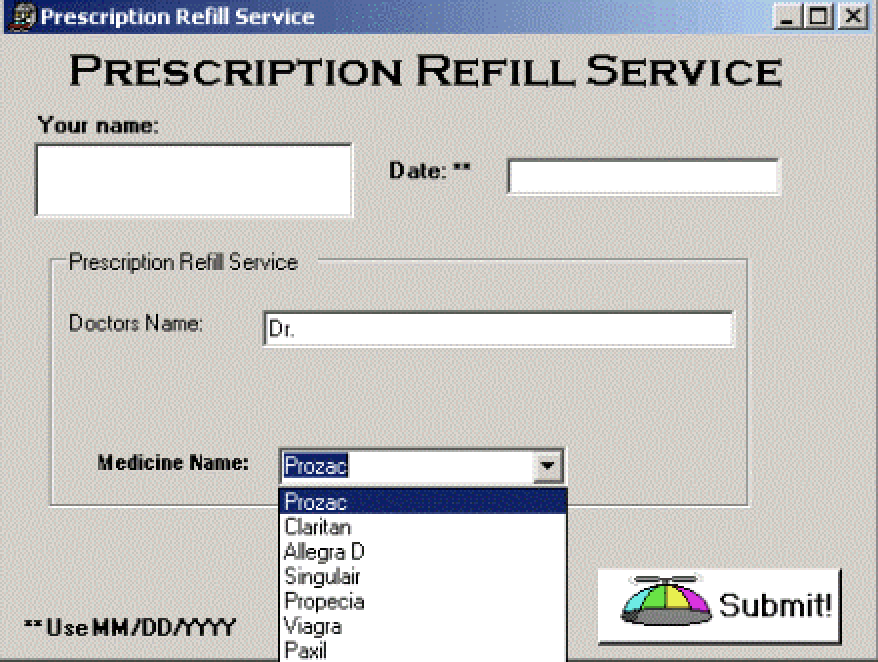
\includegraphics[width=0.5\textwidth]{1.png}
    \vspace{-1em}
\end{figure}
\end{problem}

\begin{solution}
不合理的地方:
\begin{enumerate}[label=\arabic*.]
    \item 日期不应当让用户输入:避免出错
    \item 应当使用用户听得懂得交互语言,而不是Use MM/DD/YYYY:系统与现实社会问题
    \item Submit的按钮左侧的图标没有意义:一致性和标准化
    \item 最上面的两个输入框没有对齐:标准化
    \item Your name、下拉框
\end{enumerate}

启发式设计规则:避免出错、一致化和标准化、灵活性和高效性
\end{solution}




\begin{problem}
若要将英文句子``I do like using the keystroke level model.",中的``like"替换为``hate",使之变为``I do hate using the keystroke level model."假设当前用户的手放在键盘上,且通过简单的删除和插入操作完成替换动作,应用击键层次模型对新手打字员执行该交互任务的时间进行预测。(各操作的时间见下表)
\begin{figure}[H]
    \vspace{-0.5em}
	\centering
	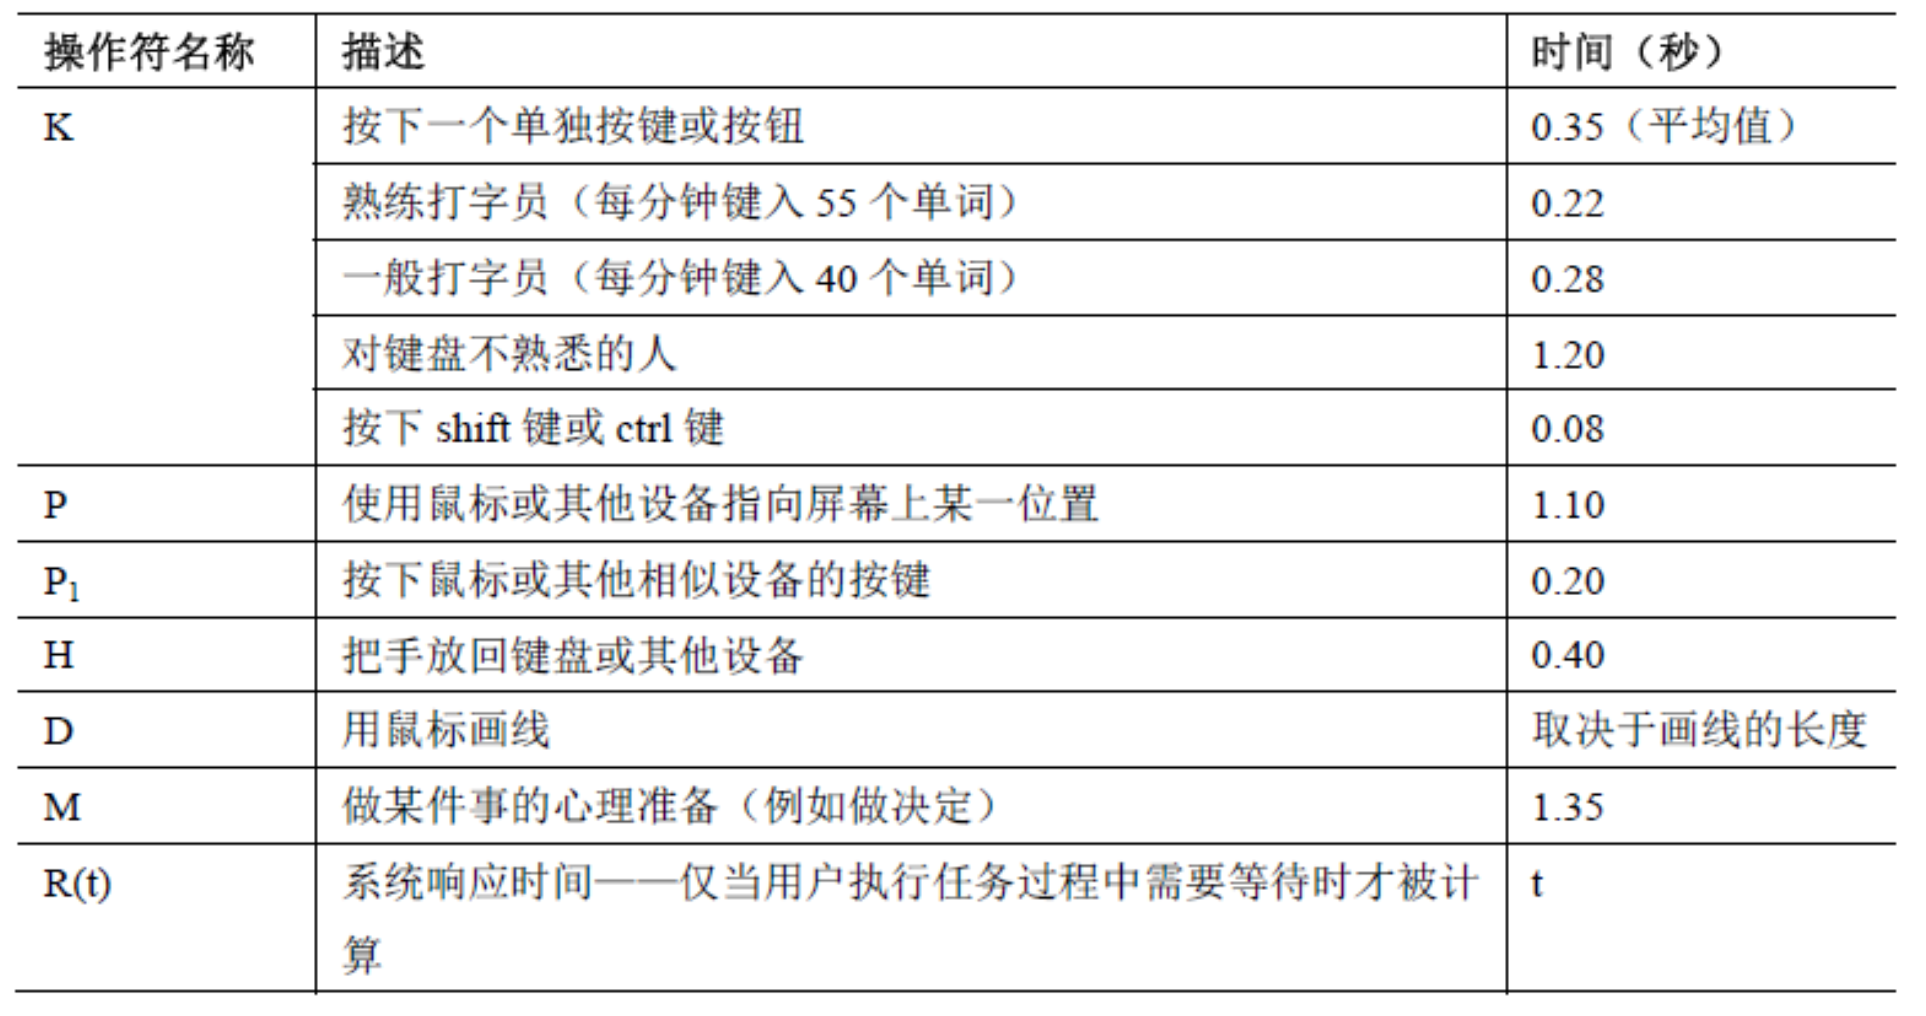
\includegraphics[width=0.7\textwidth]{2.png}
    \vspace{-1em}
\end{figure}
\end{problem}

\begin{solution}
操作序列:$M$(任务准备)、$H$(将手放在鼠标上)、$P$(将鼠标移到单词)、$P_1$(选择单词)、$H$(回到键盘)、$M$(准备键入)、$8K$(键入8下)

$T_{execute} =2\times M+ 2\times H + P +P_1 + 8\times K=7.04 (K=0.28)$
\end{solution}



\begin{problem}
随着电子商务发展越来越成熟,网上购物已经成为人们生活中的一部分,不管是衣服还是电器或者日常生活用品,选择在网上购物的人逐渐增多。请分析用户的在线购物行为,并给出该过程的层次化任务分析的文字描述和图形表示。
\end{problem}

\begin{solution}
\vspace{-0.8em}
\begin{multicols}{2}
    \begin{enumerate}[label=\arabic*.,start=0]
        \item 在线购物
        \vspace{-0.3em}
        \begin{enumerate}[label=\arabic*.]
            \item 打开在线购物软件
            \item 检索想要购买的物品
            \begin{enumerate}[label=2.\arabic*]
                \item 使用在线购物软件搜索栏
                \item 输入购买的物品的名称和特征
                \item 找出需要购买的物品
            \end{enumerate}
            \item 点开想要购买的物品的详情页面
            \item 支付并购买该物品
        \end{enumerate}
    \end{enumerate}
\end{multicols}
\vspace{-1em}

执行次序0:执行1-3-4:如果首页没有想要购买的产物品,则执行次序2-3-4
\end{solution}



\begin{problem}
可用性评估实验

\begin{enumerate}[label=\arabic*.]
    \item 目前市场上大多数移动电话都不是为老年人设计的。现在假设你需要为70岁以上的老年人设计一款移动电话,你会如何着手设计活动?需求分析阶段你将使用哪些技术?为什么?
    \item 需求分析之后,你制作了一些纸质原型,计划对他们的可用性进行评估,你将使用哪些评估方法?为什么?
    \item 假设你的设计方案被企业采纳,他们做出了一个完整的原型,并希望在开始批量生产前对其可用性进行评估。你将如何开展可用性评估?请简述评估过程。
\end{enumerate}
\end{problem}

\begin{solution}
\begin{enumerate}[label=\arabic*.]
    \item 
    \begin{enumerate}[label=(\arabic*)]
        \item 我会考虑到用户的年龄差异,提供对残缺部分的支持,更加注重容错和冗余。
        \item 技术:现场观察用户来获取同环境相关的问题。构建场景和人物角色,解决产品开发过程中出现的三个设计问题。头脑风暴等。
    \end{enumerate}
    \item 
    \begin{enumerate}[label=(\arabic*)]
        \item 快速评估、启发式评估。
        \item 在项目早期可以使用启发式评估,同时还可以结合快速评估来获取到用户的相关反馈信息。
    \end{enumerate}
    \item 
    \begin{enumerate}[label=(\arabic*)]
        \item 用户测试
        \item 选择被测试用户(三种)、开展预实验、使用DECIDE评估框架
    \end{enumerate}
\end{enumerate}
\end{solution}